\subsection{Interface thérapeutique pour l'ajustement de la difficulté de serious games}	
\emph{Hammer \& Planks} est, dans sa version thérapeutique, un jeu permettant d'aider à récupérer des facultés motrices dans le cadre d'un accompagnement à la rééducation. Rappelons qu'il s'agit d'un shooter à défilement vertical dans lequel le joueur contrôle un bateau qu'il dirige avec des mouvements du corps. Le joueur doit éviter des obstacles, affronter divers ennemis et ramasser des bonus sur la mer. Tous ces objets possèdent des attributs qu'il est possible de modifier afin d'adapter le jeu aux besoins et aux capacités du patient. Ce fut mon travail durant la première partie de mon stage de permettre de modifier ces paramètres directement à partir d'une interface web contrôlée par le soignant menant la séance de thérapie.
\paragraph{}
Ce projet se divise en deux parties distinctes~:
\begin{enumerate}
	\item L'interface thérapeutique
	\item Le paramétrage des variables de jeu
\end{enumerate}

	\subsubsection*{Interface thérapeutique}
Celle-ci permet, à partir d'un terminal distinct, de choisir un jeu et de lancer une partie sur le terminal utilisé par le patient. Ce dernier sera équipé d'un périphérique de contrôle comme la caméra Kinect ou la wii board. A partir de cette interface, le soignant est en mesure de voir et de modifier l'ensemble des paramètres de jeu (en tout cas, le sous-ensemble considéré comme pertinent et effectivement envoyé à l'application). De plus, à la fin d'une partie, il sera capable de visualiser les données de la session de jeu, comme l'apparition d'évènements ou les zones que le joueur a réussi ou non à atteindre. Ces informations sont utiles pour mieux cibler les difficultés du patient et ajuster au mieux les prochaines séances. Cette partie du projet a été réalisée par Andy Camicci durant son stage chez NaturalPad entre Avril et Juin 2013.

\begin{figure}[htbp]
	\centering
%	\includegraphics[scale=]{images/interface_therapeutique_01.png}
	\caption{TODO Modification des valeurs du jeu dans l'interface thérapeutique}
	\label{interface_therapeutique_01}
\end{figure}

\begin{figure}[htbp]
	\centering
%	\includegraphics[scale=]{images/interface_therapeutique_02.png}
	\caption{TODO Visualisation des données de la partie.}
	\label{interface_therapeutique_02}
\end{figure}

	\subsubsection*{Maitriser la difficulté : le paramétrage des variables de jeu}
Cette partie consiste en l'extraction des paramètres de jeux et en la création d'un système permettant de créer, d'enregistrer et de transmettre des configurations de ces attributs à l'interface thérapeutique.

\paragraph{}
\emph{Hammer \& Planks} est développé avec le moteur de jeu Unity3d et les scripts codés avec le langage de programmation C\#. Comme nous l'avons dit, \emph{H\&P} possède de nombreux contenus contribuant à la richesse du gameplay et aux possibilités d'ajustement. Lors de mon arrivée au sein de NaturalPad, ces objets n'étaient cependant pas ajustables facilement : il fallait rechercher l'ensemble des objets dont on souhaitait modifier un paramètre, trouver les variables correspondant à ces paramètres puis les modifier soit directement dans le code soit par l'intermédiaire de l'éditeur d'Unity. La raison en est que les contraintes de développement du jeu n'ont pas permis de découpler ces informations.

\paragraph{}
Mon premier travail a donc été de découvrir le code et de rechercher toutes les variables dont on souhaiterait potentiellement vouloir modifier la valeur dans un contexte d'ajustement du jeu pour un exercice de rééducation. J'ai ensuite créé une classe spécifique permettant de regrouper conceptuellement les données modifiables. J'ai ainsi regroupé ces données dans des thèmes tels que \emph{réseau}, \emph{ennemis}, \emph{joueur}, \emph{contrôles} ou \emph{cosmétiques}.

\paragraph{}
En parallèle, j'ai aussi procédé au refactoring de l'ensemble des classes possédant ou utilisant un ou plusieurs attributs modifiables. L'intérêt était bien sur d'avoir un accès commun unique à ces valeurs, mais aussi et surtout que les valeurs puissent être modifiées de manière extérieure par l'interface thérapeutique. Par ailleurs, la modification de ces valeurs par l'interface devait être certaine et pérenne, afin que les modifications apportées soit effectivement prises en compte par l'application et donc modifier l'expérience de jeu en direct.

	\subsubsection*{Préparer l'évolution du jeu et de la séance}
Si permettre un ajustement en direct des propriétés du jeu par le soignant était une fonctionnalité que nous voulions impérativement mettre en place, celle-ci peut se révéler contraignante et répétitive si elle est utilisée seule. Nous voulions ainsi la possibilité de pouvoir enregistrer des configurations de paramètres, afin de pouvoir passer de l'une à l'autre aisément sans devoir faire chaque modification séparément. Par ailleurs, cela permet d'envisager beaucoup de possibilités comme la personnalisation de configurations pour des patients, l'adaptation aisée du jeu pour des besoins thérapeutiques différents ou encore l'automatisation d'une progression de la difficulté à l'aide de configuration prédéfinies.

\paragraph{}Afin d'utiliser des fichiers de configurations, il a fallu créer un système permettant de serialiser les données puis de les charger et de les lier à l'instance de jeu.\\
J'ai par ailleurs durant mon stage créer plusieurs fichiers de configuration permettant une évolution progressive de la difficulté dans le mode de jeu Survie de \emph{Hammer \& Planks}, pour sa version grand public.

	\subsubsection*{Usage : tests, retours et intégrations}
Si le projet \emph{Hammer \& Planks} a été initié par une étudiante en ergothérapie, il est aussi et surtout développé en collaboration avec le pôle de rééducation du centre hospitalier de Lapeyronie à Montpellier. Comme nous l'avons dit, le projet a évolué et son champs d'action, en plus d'un travail sur l'équilibre, s'étend maintenant à de l'aide à la rééducation des membres supérieurs, du tronc et du bassin. Le travail d'équilibre, qu'il soit debout ou assis, s'effectue en utilisant la balance de la Wii, qui enregistre les changements du centre de gravité du joueur-patient pour contrôler le bateau. L'intégration d'un contrôle avec la Kinect permet au joueur d'utiliser d'autres mouvements de son corps. Il est ainsi possible d'utiliser son bras ou sa main pour diriger le bateau, ou les mouvements du tronc et du bassin que ce soit en position assise ou debout.

\paragraph{} Nous approchant d'une méthode de conception participative, nous avons ainsi réalisé plusieurs séances de tests avec des patients hémiplégiques et leurs thérapeutes. \\
Les premières choses marquantes sont la curiosité et l'enthousiaste général à la fois des patients et du personnel soignant. Peu d'entre eux connaissaient l'existence de jeux sérieux pour la santé, et dans le cas contraire, appréciaient particulièrement l'accent mis sur l'aspect vidéo-ludique de \emph{Hammer \& Planks}. Ce fut donc un premier point très positif pour l'équipe.

\paragraph{} 
Lors de la première séance de tests, nous avons ainsi eu de nombreux retours positifs portant sur la possibilité d'ajuster le jeu en direct, la visualisation des informations de la session de jeu ou encore le plaisir de jeu. Nous avons aussi eu de nombreuses remarques menant à l'ajout de fonctionnalités, notamment par le personnel.\\
Les remarques les plus fréquentes concernaient le visuel du jeu : les soignants craignaient que les graphismes soient trop riches et les effets trop complexes pour des patients hémiplégiques. L'effet visuel des mouvements de la mer fut notamment cité, et la différenciation entre bonus et obstacles (ennemis, projectiles et mines ennemies) jugée trop complexe.\\
Enfin, réaliser des tests pendant une demie-journée nous a aussi permis de juger notre travail de manière différente. Nous avons ainsi remarqué que nous faisions régulièrement voir systématiquement certains ajustements de paramètres, alors que certaines valeurs n'étaient jamais utilisées.

\paragraph{De l'importance des tests utilisateurs\\}Petite anecdote enfin, prouvant définitivement l'importance de réaliser des tests en conditions réelles. Lorsqu'on utilise le jeu avec la Kinect, le joueur doit lever la main afin d'être reconnu comme la personne joueuse parmi les possibles multiples personnes détectées par la caméra. Ce système fonctionnait parfaitement lors de nos test en interne. Or quand une patient hémiplégique a tenté de jouer, le système ne la reconnaissait pas. La raison en était que la patiente avait une hémiplégie du coté gauche et voulait donc jouer avec sa main gauche pour travailler sa rééducation. Or, le système était configuré pour ne détecter qu'une main droite... aucun membre de l'équipe n'étant gaucher, nous n'avions pas détecté ce grossier oubli ! L'erreur a bien sur depuis était corrigée.

	\paragraph{\emph{Intégration}\\}
	Forts de ces retours, nous avons ensuite classé les remarques qui nous été faites et celles que nous avons notées. Puis, nous avons discuté de la pertinence et de l'importance de chacune d'elle, ainsi que des différentes possibilités d'y répondre. \\
	Concernant la surcharge visuelle, pouvant poser des problèmes cognitifs à certains patients, surtout pour des personnes peu voir pas habituées aux jeux vidéo, nous avons mis en place la possibilité d'ajuster les paramètres visuels. Il est possible de modifier le contraste du jeu, la taille des éléments interactifs ou encore de supprimer les objets cosmétiques (requins, mouettes, brouillard, effet de la mer, etc.). Nous avons par ailleurs augmenté la taille des projectiles (ennemis et alliés) et ajouté un effet de trainée, les rendant beaucoup plus visibles.\\
	Concernant les bonus, jugés trop difficiles à ramasser, nous mis en place deux systèmes. Le premier est la possibilité de mettre un halo vert autour des différents bonus, les rendant bien plus visibles. Le second, est un mécanisme d'aimantage des bonus vers le bateau du joueur. Cette attraction, dont le rayon est ajustable dans les settings, permet de récupérer les bonus même si on ne passe pas directement dessus, ce qui est souvent difficile et frustrant pour le joueur.\\
Concernant les paramètres enfin, nous modifié les valeurs par défaut de certains et ajuster les bornes min et max des plages de valeurs.

		
	\paragraph{} Nous avons ensuite réalisé une nouvelle séance de tests du jeu intégrant ces modifications. C'est avec plaisir que nous avons constaté que les réponses apportées étaient pertinentes et plaisaient à nos testeurs. Ce fut aussi l'occasion d'avoir de nouveaux retours et de continuer notre processus de conception participative.
	
\paragraph{montrer un aperçu des valeurs modifiables?} et leur utilité d'un point de vue
ajustement et rééduc. Et peut être aussi des images sur le thème "avant/après" pour montrer l'évolution et l'intéret des test en situation.

	\subsubsection*{Conclusion}
	Cette expérience et ce travail sur \emph{Hammer \& Planks} m'ont permis de vérifier l'intérêt et la réelle pertinence de jeux sérieux pour la rééducation. Par ailleurs, l'intégration d'un nouveau périphérique, la Kinect, débloquant de nouveaux gameplay avec un système de jeu identique, m'a confirmé l'importance du moyen de contrôle à la fois sur le gameplay mais aussi et surtout sur la richesse des applications thérapeutiques qui en découle. Enfin, les critiques des soignants et des patients au cours des deux séances de tests m'ont assuré de l'importance et du réel intérêt de pouvoir ajuster manuellement les variables de jeux directement pendant la séance. C'est à la fois très gratifiant pour notre travail et très encourageant pour les possibilités en terme de réhabilitation.
	
\paragraph{}
Cependant, un seul jeu, aussi ajustable soit il, ne peut suffire à répondre à tous les besoins et cas d'utilisation. Il y a trois aspects~:
\begin{enumerate}
	\item le cœur du jeu, qui décrit ses lois, objectifs et règles de fonctionnement. Il est propre au jeu (ou à un type de jeu) et non modifiable.
	\item les variables ajustables, qui ne modifient pas les règles mais définissent entre autres la difficulté.
	\item le gameplay, induit par les deux premiers points ainsi que par les périphériques et méthodes de contrôle utilisés. En général, ces derniers sont pris en compte dès l'établissement du coeur du jeu, certaines associations étant incompatibles.
\end{enumerate}
\paragraph{}
Il est possible de modifier l'expérience de jeu en modifiant la valeur des variables ajustables : c'est ce que nous proposons à l'aide de notre interface thérapeutique. Il est aussi possible d'explorer un gameplay a priori identique avec des contrôleurs différents, rendant ainsi à la fois l'expérience de jeu et les mouvements induits différents.
\\Cependant, même ainsi, un jeu vidéo avec un coregame propre finit par montrer ses limites en terme d'adaptation, et il est alors nécessaire de proposer d'autres types de jeux vidéo si l'on veut explorer de nouvelles pistes de rééducation.\\
Pour cette raison, toujours dans l'idée d'une adaptation de la difficulté, la suite logique était de proposer une méthode permettant d'aider à la conception de jeux sérieux thérapeutiques.
 
\subsection{Conception}
	La seconde partie de mon travail fut donc consacrée à la proposition et à l'expérimentation de moyens de conception de jeux vidéo sérieux pour la santé. Pour cela, j'ai en fait emprunté deux approches, répondant à des contextes un peu différents.
	
	\subsubsection{Ensemble d'outils d'aide à la conception de SG}
	La première proposition s'inscrit dans une problématique où l'on souhaiter créer un serious game dont l'objectif sérieux est de l'ordre de l'aide à la réhabilitation motrice. Il s'agit ici de proposer un outil intégrant un certain nombre de connaissances utiles ou nécessaires à la conception de ce type de jeux. L'idée est de mettre à disposition des documents regroupant un maximum des informations qui seront utiles dans le processus de conception. Cela permettrait aux différents corps de métier impliqués dans le processus de conception d'avoir accès aux connaissances qui leur font défaut et d'avoir une vision globale des éléments en jeu.
	
		\paragraph{}
A la frontière entre conception de jeux vidéo et monde médical, ce travail nécessite la compétence de professionnels de la santé ainsi que d’une expertise du domaine du jeu vidéo.
			\paragraph{\emph{Aspect médical}\\}
La première étape consiste à définir et lister les objectifs thérapeutiques que l’on souhaite atteindre, les exercices que proposent les professionnels pour y parvenir, ainsi que les éléments de difficulté qui peuvent être rencontrés dans ces exercices. Ces informations doivent provenir de médecins et de thérapeutes qui vont trouver un intérêt dans l’utilisation ou la prescription de serious games pour la santé. Les informations que j'ai pu recueillir, particulièrement autour de l'AVC, sont regroupées dans la partie \ref{objectifs_therapeutiques}.

\paragraph{}
Dans le but de faciliter la démarche de conception en fonction d’un objectif thérapeutique particulier, il est aussi intéressant de trouver une méthode classification de ces objectifs qui soit parlante pour les thérapeutes. Dans le cadre de mon stage, je me suis particulièrement concentré sur les aspects moteurs, comme présenté dans la figure \ref{objectifs_moteurs}. Pour réaliser ce document, je me suis tout d'abord inspiré de mes recherches documentaires et du résultats de mes différents entretiens avec des professionnels de la santé.

\paragraph{}
Dans cette première version, j'avais classé les objectifs thérapeutiques au moyen de trois propriétés : la zone du corps affectée (membres supérieurs, inférieurs, tête, tronc), le membre précisément affecté (main - poignet- avant-bras ou pied - jambe, etc.) et des paramètres propres à ces membres (amplitude, force, vitesse ou durée de mouvements, membre gauche ou droit, etc.). Cependant, cette première version avait l'inconvénient de proposer des éléments différents selon le choix initial, et d'autres éléments étaient dupliqués.

\paragraph{}J'ai ensuite proposé ma classification à deux kinésithérapeutes (Didier Costeau et Karima Bahkti) afin de voir si elle leur semblait pertinente ou s'ils voyaient des éléments à ajouter ou à modifier. Il s'est en fait avéré que cette classification ne correspondait pas du tout à la manière dont raisonnent les thérapeutes lorsqu'ils établissent les objectifs d'une rééducation. Ce fut donc l'occasion de re-designer cette classification. La version 2 ici proposée en figure \ref{objectifs_moteurs} a par la suite été revue et validée.

\paragraph{}Par ailleurs, dans la perspective d'étendre la portée de l'outil, j'ai aussi ébauché une proposition de listing d'objectifs thérapeutiques de différents types, présentée dans la figure \ref{objectifs_autres}.

\begin{figure}[hbtp]
	\centering
	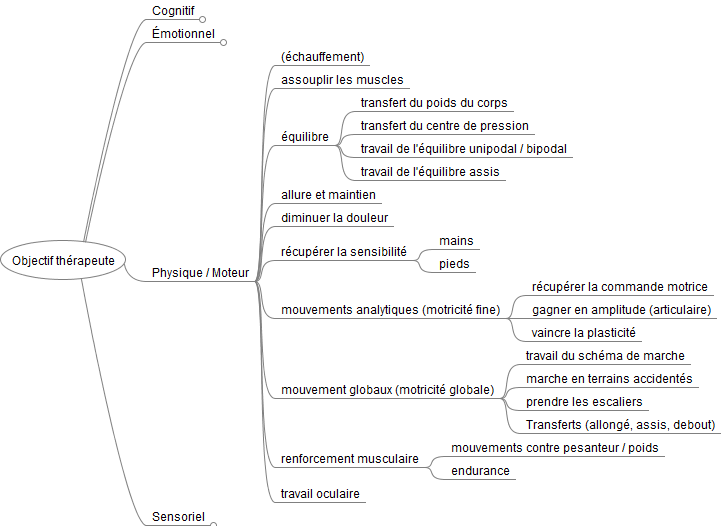
\includegraphics[width=16cm]{images/objectifs_moteurs}
	\caption{Listing et hiérarchisation des objectifs thérapeutiques moteurs}
	\label{objectifs_moteurs}
\end{figure}

\begin{figure}[hbtp]
	\centering
	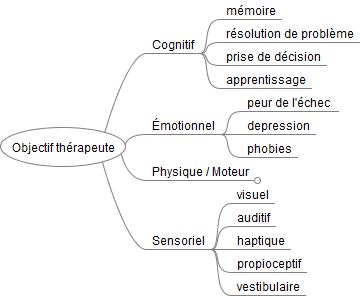
\includegraphics[scale=0.7]{images/objectifs_autres}
	\caption{Ébauche de classification de différentes types d'objectifs thérapeutiques}
	\label{objectifs_autres}
\end{figure}

			\paragraph{\emph{Aspect Game Design}\\}
L'autre aspect du processus de conception de serious games pour la santé concerne l'aspect vidéo-ludique. Pour cela, j'ai tout d'abord commencé par établir une classification des principaux types de jeux vidéo en fonction de leur gameplay, visible dans l'annexe \ref{types_jeux}. Ce document peut être intéressant pour plusieurs raisons. Dans un premier temps, il peut permettre aux concepteurs d'envisager des gameplays auxquels ils n'auraient pas pensé : par oubli ou simplement par méconnaissance du concept de jeu. Pour être plus parlante, la classification propose par ailleurs des exemples de jeux existants pour chaque type de gameplay. \\
Bien sur, cette liste ne peut être totalement exhaustive : beaucoup de jeux vidéo, particulièrement les jeux mettant l'accent sur une difficulté logique, possèdent leur style propre.

\paragraph{}
De l’autre coté du processus, il est nécessaire d’établir le lien entre les différents types de jeux vidéo existant, leur gameplay et les types de contrôles qui s’y adaptent de manière optimale. Un dernier élément, en lien avec les éléments de difficulté d’un jeu, est l’ajustement de la difficulté et l’évolution possible de celle-ci, en terme de gameplay. La littérature et l’analyse des jeux vidéo existant peuvent aider à connaître ces liens. 

			\paragraph{\emph{Le contrôle, lien entre objectifs thérapeutiques et contraintes ludiques}\\}
L’objectif sérieux des serious game étant de nature motrice, nous avons décidé de nous concentrer sur les contrôles. Pour faire le lien entre les objectifs thérapeutiques et le jeu sérieux que l’on veut créer pour y répondre, l’utilisation d’interface dites naturelles comme la Kinect ou les accessoires de la Wii nous semblait particulièrement pertinente. Nous souhaitons alors orienter la conception du jeu pour qu’il utilise l’un de ces outils afin de permettre le contrôle qui correspond le plus naturellement aux exercices que l’on cherche à faire réaliser par le joueur-patient. Il est nécessaire pour cela de trouver comment adapter les contrôles classiques d’un gameplay donné en contrôles naturels, cad, comment passer de la manette à un contrôle par les gestes pour chaque type de gameplay.

	
	\subsubsection{Proposition d'une méthodologie de conception de SG}
	\paragraph{}
	deuxieme propo c'est de faire comme j'ai fait avec impact mapping et al.
	
	  j'ai ma mind map des objectifs thérapeutiques d'ordre moteurs, mais d'un autre, on a quand meme (évidemment) refait une séance de coconception à la fois avec arnaud et les ergo/kine d'ales. il y  aussi les propositions de controles NUI pour les jeux classiques, en parlant du fait de se restreindre a certain périphériques ; et le classement des types de jeux.
	 
 Le pb c'est que j'ai rien qui dise clairement "pour tel exercice/objectif, fais plutot ce type de jeu avec tels contrôles. Du coup, est-ce que ca pourrait pas être une forme de perspective? disant que ça nécessiterait du travail et serait moins parfait qu'un truc personnalisé, mais ca permettrait de gagner du temps tout en étant mieux que ce qui existe actuellement. A l'inverse, la démarche que j'ai emprunté dans ma méthode semble mieux coller aux besoins, mais nécessite plus de travail.
 
 bien expliquer si ces démarches sont différentes, complémentaires ou partiellement complémentaires, dans quels contextes elles s'appliquent et quels sont les compétences nécessaires à quels moments pour les mettre en place.
 Pensez aux perspectives de l'ordre de "ca serait bien d'éprouver la méthodologie sur un projet complet" , "il faudrait une équipe avec telles compétences"
		\subsubsection{}

	*conception participative avec Arnaud 
		-impact mapping, carte d'empathie et scénarios d'usage et storyboard
	*séance de conception participative à Alès (Rhabdomyolyse)
	
	-travail avec les thérapeutes
	-répondre aux objectifs thérapeutique par un gamedesign
		- hammer \& Planks et l'équilibre (voir rapport d'anais)
		- classement des objectifs thérapeutique, carte d'impact
	-ajustement de la difficulté et lien avec la thérapie : impact des paramètres en terme de difficulté (équilibre et dos?)
	
	-proposition de controle naturels pour des jeux pour une utilisation thérapeutiques